\documentclass[11pt]{article}
    \usepackage{caption}
    \usepackage{graphicx}
    \usepackage{mathtools}
    \usepackage{bookmark}
    \graphicspath{ {img/} }
    \setlength{\parindent}{0pt}
    \DeclareCaptionType{equ}[][]
    \usepackage[svgnames]{xcolor}
    
    \newcommand*{\plogo}{\fbox{$\mathcal{BM}$}}
        
    \usepackage{PTSerif}
    
    \begin{document} 
        
    \begin{titlepage}
    
        \raggedleft
        
        \vspace*{\baselineskip}
        
        {\Large Bryan Melanson}
        
        \vspace*{0.167\textheight}
        
        \textbf{\LARGE How to Not Fail}\\[\baselineskip]
        
        {\textcolor{Red}{\Huge Electronic Circuits II}}\\[\baselineskip]
        
        {\Large \textit{While never going to class}}
        
        \vfill
        
        {\large Computer Engineering 2020 ~~\plogo}
        
        \vspace*{3\baselineskip}
    
    \end{titlepage}

    \pagebreak
    
%%%%%%%%%%%%%%%%%%%%%%%%%%%%%%%%%%%%%%%%%%%%%%%%%
    \pdfbookmark[section]{\contentsname}{toc}

    \tableofcontents


    \pagebreak
%%%%%%%%%%%%%%%%%%%%%%%%%%%%%%%%%%%%%%%%%%%%%%%%%

    
    \section{Operational Amplifiers}
    An \textit{Operation Amplifier} is a device which, when powered by $+V$ and $-V$ DC power sources, will amplify an input signal with infinite gain. The input terminals are known as the \textit{non-inverting} ($+$) and \textit{inverting} ($-$) terminals.

    Where no input current enters $+$ and $-$, and the \textit{input impedance is infinite.}
\begin{center}
    \begin{figure}[h]
        \centering
        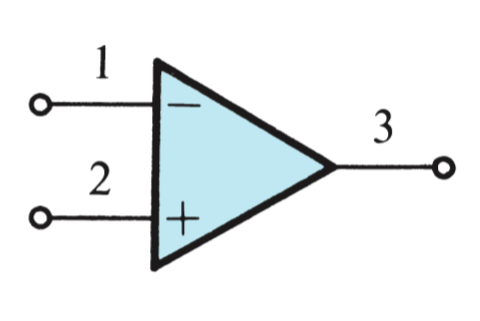
\includegraphics[width= 200 px]{op}
        \caption{Ideal Op Amp}
        \label{fig:op amp}
    \end{figure}
\end{center}
    

    $A$ is referred to as the \textbf{Open Loop Gain}, where the output and inputs have not been connected. The \textbf{Closed Loop Gain} will be denoted as $G$. \\ 

    The \textbf{Differential Input Signal} $v_{id}$ and \textbf{Common Mode Input Signal} $v_{Icm}$ are two signals that define the operation of the op-amp. Because the op-amp is designed to detect the difference between two signals, they are denoted as the term $v_id$. The op-amp will also reject common signals, because only the difference between the two signals will be used for output.

    \begin{center}
        $v_{id} = v_2 + v_1$ \\
        $v_{Icm} = \frac{1}{2}(v_1 + v_2)$ 
    \end{center}

    \subsection{Inverting Configuration}

    In the inverting configuration, the output of the op-amp is connected back into the inverting terminal. Because in the inverting configuration $v_2$ is grounded, the negative output counteracts the inifite gain and \textit{closes the loop} around the op amp so that it provides a stable output. \\
    
    In the case where a resistance is placed between $v_2$ and $v_o$, there would be a \textbf{Positive Feedback}, and the output would increase exponentially.
   
    \begin{figure}[h]
        \centering
        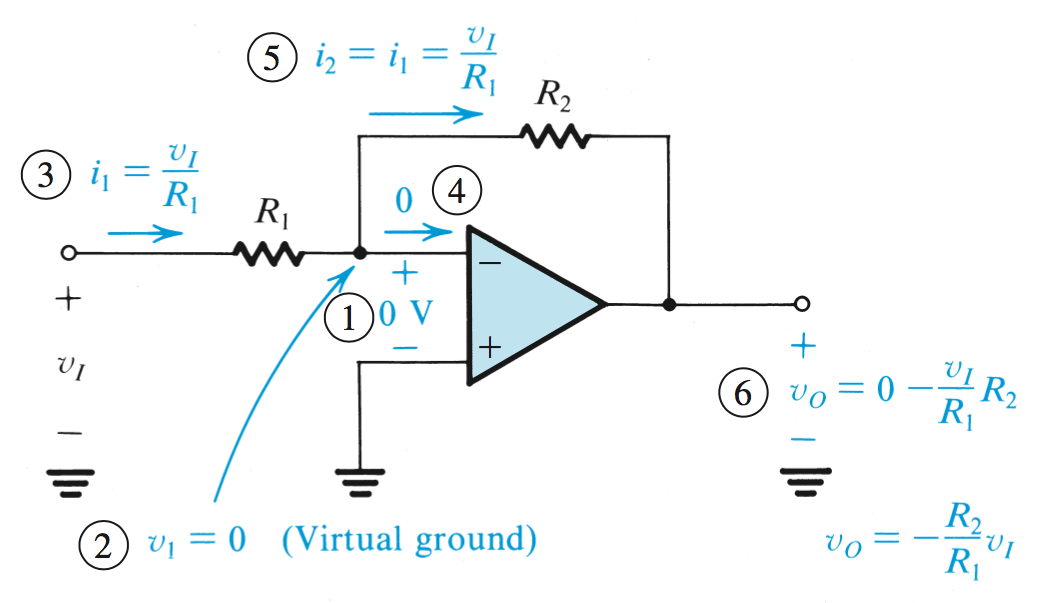
\includegraphics[width=\textwidth]{invert}
        \caption{Inverting Configuration of Op Amp}
        \label{fig:inverting }
    \end{figure}

    \begin{center}
        $v_3 = A(v_2-v_1)$
    \end{center}

    If $v_2 = v_1$, the output will be $0$. Where A is infinite,

    \begin{center}
        $\frac{v_3}{A} = v_2-v_1$ \\
        
        $0 = v_2-v_1$

        $v_2 = v_1$
    \end{center}

    This is known as a \textit{Virtual Short Circuit}. \\
    
    The \textbf{Closed Loop Gain} $G$ is defined as $\frac{v_o}{v_i}$ \\
    
    From Figure 1, we can see that knowing $v_1 = v_2 = 0$, therefore $i_1$ can be calculated, and passes to the input without entering the op amp terminals. \\
    
    \begin{equ}[!ht]
        \begin{equation}
            G = \frac{v_0}{v_i} = -\frac{R_2}{R_1}
        \end{equation}
      \caption{Closed Loop Gain of a Non-Inverting Amplifier}
    \end{equ} 
    
    \subsubsection{Finite Open-Loop Gain}
    When the open-loop gain $A$ is not finite, $\frac{v_3}{A} = v_2-v_1$ no longer produces $v_2 = v_1 = 0$, instead $v_2 = v_1 = \frac{v_o}{A}$. Knowing this, calculations for $i_1$ will follow the same logic, instead with accounting for $\frac{v_0}{A}$.
    \subsubsection{Input and Output Resistance}
    The input resistance is equal to $R_1$, and the output resistance is $0$.
    \subsubsection{Weighted Summer}
    In this configuration, $i$ will be the sum of all incoming currents. Therefore, 
    
    \begin{center}
        $i = \frac{v_1}{R_1} + \frac{v_2}{R_2} + ...$ \\
    \end{center}

    In the case where a design must be created to fit an equation with multiple inverted signs, two op-amps can used in series to flip the initial signals.

    \begin{center}
        $v_o = v_1(\frac{R_a}{R_1})(\frac{R_c}{R_b}) + v_2(\frac{R_a}{R_2})(\frac{R_c}{R_b}) - v_3(\frac{R_c}{R_3}) - v_4(\frac{R_c}{R_4})$
    \end{center}

    \begin{figure}[h]
        \centering
        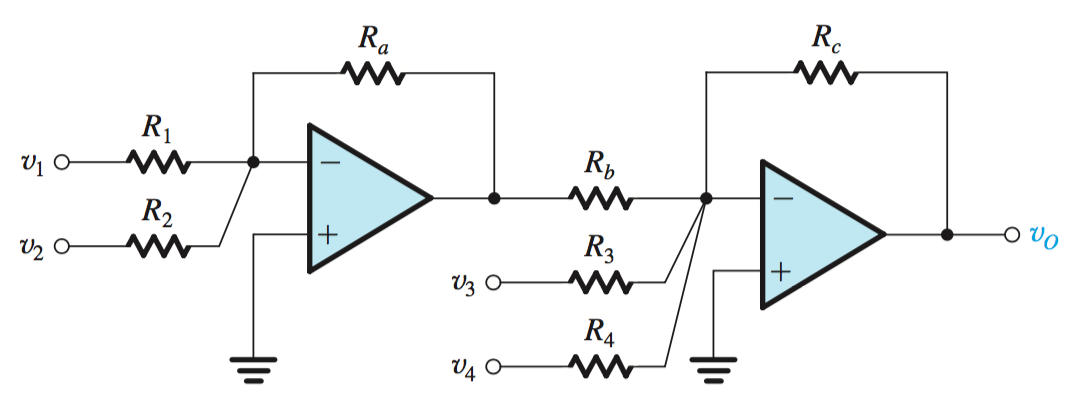
\includegraphics[width=\textwidth]{summer-2}
        \caption{Weighted Summers in Series}
        \label{fig:weight summers}
    \end{figure}

    \subsection{Non-Inverting Configuration}

    The Non-inverting configuration occurs when a voltage input enters the $v_2$ terminal, instead of $v_1$, while the resistor loop configuration is identical. As with the other closed loop, there is a virtual short circuit between $v_2$ and $v_1$, therefore $v_2 = v_1 = v_I$, the applied voltage. \\
    
    The $v_1$ terminal, grounded in this case, creates $i_1 = \frac{v_I}{R_1}$, and the solution can follow as before.

    \begin{equ}[!ht]
        \begin{equation}
            G = \frac{v_0}{v_i} = 1 + \frac{R_2}{R_1}
        \end{equation}
      \caption{Closed Loop Gain of a Non-Inverting Amplifier}
    \end{equ}
    
    \subsubsection{Finite Open-Loop Gain}

    When the open-loop gain $A$ is not finite, $\frac{v_3}{A} = v_2-v_1$ no longer produces $v_2 = v_1 = 0$, instead $v_2 = v_1 = \frac{v_o}{A}$. Knowing this, calculations for $i_1$ will follow the same logic, instead with accounting for $\frac{v_0}{A}$.

    \subsubsection{Buffering Amplifier or Voltage Follower}
    
    In this configuration, the loop is closed by short circuiting the output to non-inverting input. This will again create a virtual short circuit between $v_2$ and $v_1$, and because a real short circuit exists between $v_1$ and $v_o$, all terminal values will be equal to the voltage source, $v_I$. \\
    
    \begin{figure}[h]
        \centering
        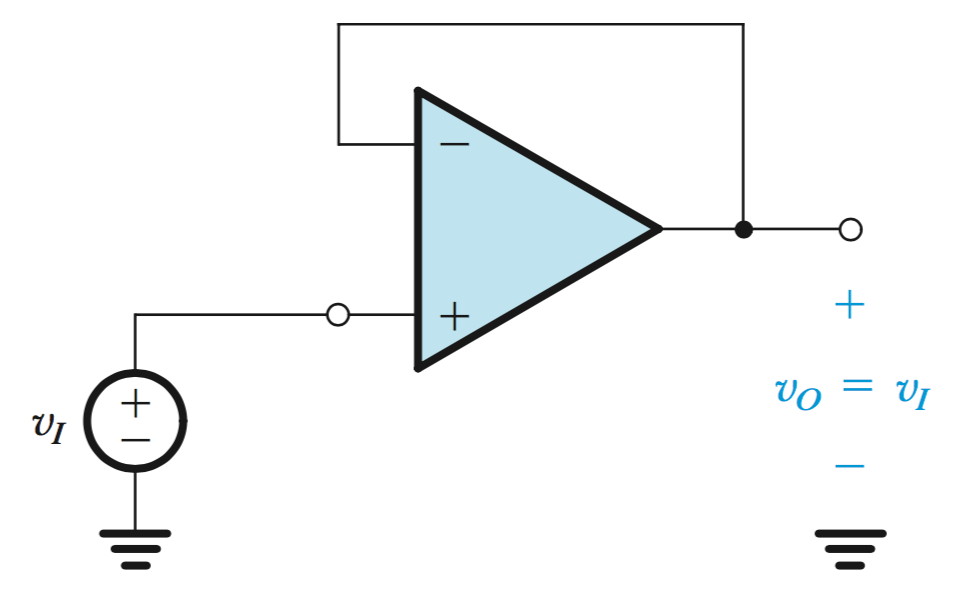
\includegraphics[width=\textwidth]{buff}
        \caption{Buffer Amplifier or Voltage Follower}
        \label{fig:voltage follower}
    \end{figure}

    \subsection{Difference Amplifiers}
    A Difference Amplifier is one where voltage sources are applied to the $v_2$ and $v_1$ inputs. The output can then be considered a non-inverting configuration and an inverting configuration superimposed on each other. By using supoerposition, the effect of each voltage source can then be calculated separately and summed together independent of one another. \\

    In a case like this, $v_o = A_dv_{id} + A_{cm}v_{Icm}$, and the efficiency of the Difference Amplifier can be determined by its \textit{common-mode rejection ratio (CMRR)}

    \begin{equ}[!ht]
        \begin{equation}
            \text{CMRR} = 20 \text{log}\frac{|A_d|}{|A_{cm}|}
        \end{equation}
      \caption{Common Mode Rejection Ratio}
    \end{equ}

    In a Difference amplifier with voltage sources at $v_2$ and $v_1$, it can be seen that this will have a inverting and non-inverting output superimposed on one another. However, the gain ratio of both inputs must be equal for the common mode ratio rejection, so the $v_2$ input must use a voltage divider ($v_3$ and $v_4$) to reduce the input voltage.\\
    
    Therefore, $\frac{R_4}{R_4 + R_3}(1 + \frac{R2}{R1}) = \frac{R2}{R1}$, and $\frac{R4}{R3} = \frac{R2}{R1}$. \\

    To find values concering solely the $v_{Id}$ and $v_{Icm}$, consider a voltage source $v_Id$ or $v_Icm$ applied at the inputs, where $v_Icm$ is applied to both, and the negative and positve termals of $v_{id}$ are connected in series between the two terminals.

    \begin{figure}[h]
        \centering
        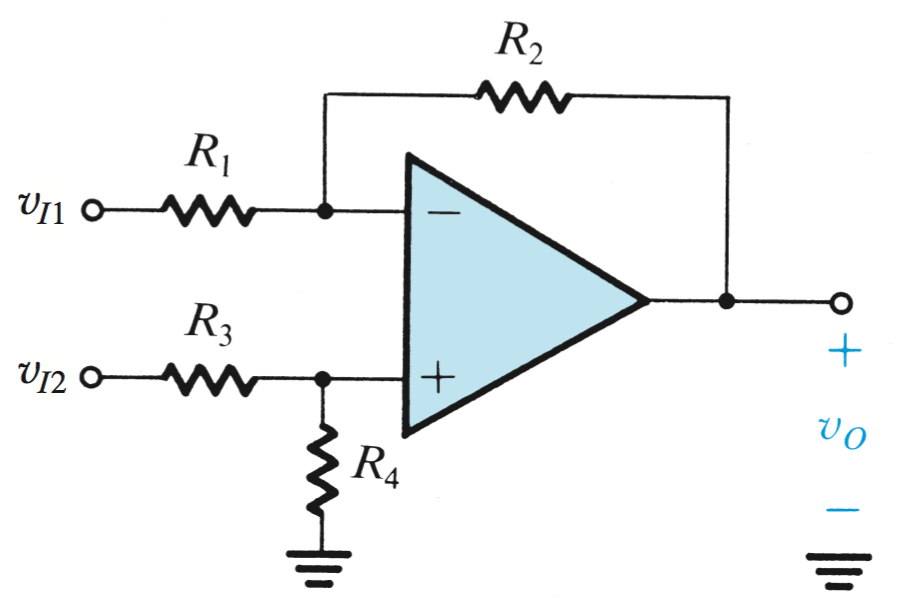
\includegraphics[width=\textwidth]{diff}
        \caption{Difference Amplifier}
        \label{fig:difference amplifier}
    \end{figure}

    \subsubsection{Instrumentation Bridge Amplifiers}

    The Instrumentation Bridge Amplifier is a Difference Amplifier created as a solution to the low input resistance of Difference Amplifiers, without sacrificing ease of control. From Figure 6, it can be noted that $R_1$ can be used to control the output voltage of the circuit.
    
    \begin{equ}[!ht]
        \begin{equation}
            v_o = \frac{R4}{R3}(1 + \frac{R_2}{R_1})v_{Id}
        \end{equation}
      \caption{Output of the Instrumentation Bridge Amplifier}
    \end{equ}

    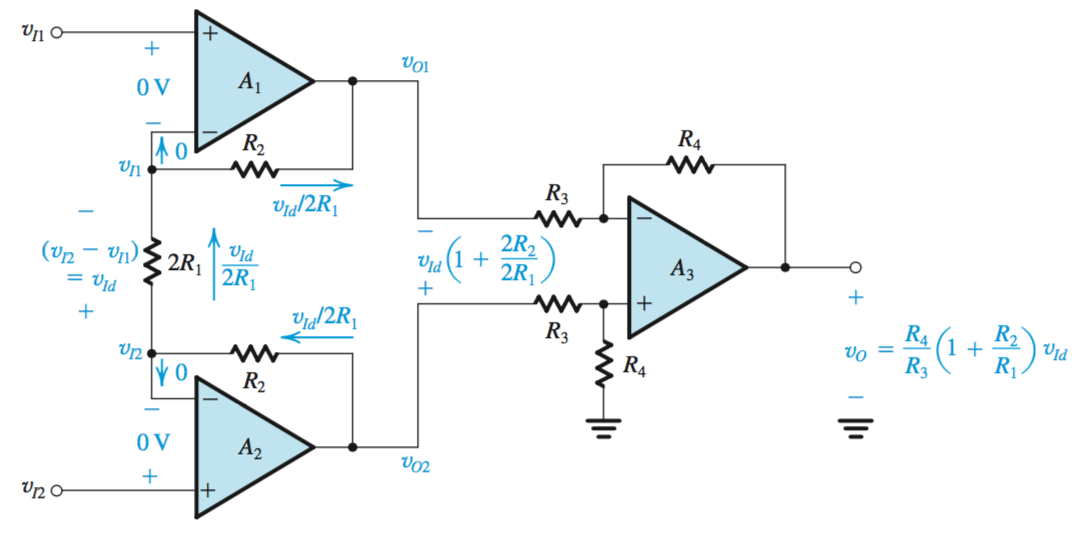
\includegraphics[width=\textwidth]{instr}

%%%%%%%%%%%%%%%%%%%%%%%%%%%%%%%%%%%%%%%%%%%%%%%%%

    \section{Filters and Tuned Amplifiers}
    A filter is a linear two-port network with a transfer function $T(s) = V_o(s)/V_i(s)$. For physical frequencies, the filter transmission is expressed as $T(j\omega) = |T(j\omega)|e^{j\phi(\omega)}$. The magnitude of transmission can be expressed in decibels using either the gain function $G(\omega) = 20\text{log}|T|$ or the attenuation function $A(\omega) = −20 \text{log} |T|$.    \\
    
    \textbf{Note on Imaginary Numbers} \\
    
    Magnitude = $\sqrt{\Re^2 + \Im^2}$ \\

    $|\frac{\omega_0}{\omega_0+\omega j}| = \frac{\sqrt{\omega_0 ^2}}{\sqrt{\omega_0^2 + \omega^2}} = \frac{\omega_0 ^2}{\sqrt{\omega_0^2 + \omega^2}}$ \\
    
    Phase = $\text{tan}^{-1}(\Im / \Re)$ \\
    
    $\phi(\frac{\omega_0}{\omega_0+\omega j}) = \frac{\text{tan}^{-1}\frac{0}{\omega_0}}{\text{tan}^{-1}\frac{\omega}{\omega_0}}$
    
    \subsection{Filter Transmission}

    The transmission characteristics of a filter are specified in terms of the edges of the passband(s) $\omega_p$ and the stopband(s) $\omega_s$. The maximum allowed variation in passband transmission, $A_{max}$ (dB); and the minimum attenuation required in the stopband, $A_{min}$ (dB). In some applications, the phase characteristics are also specified. \\
    
    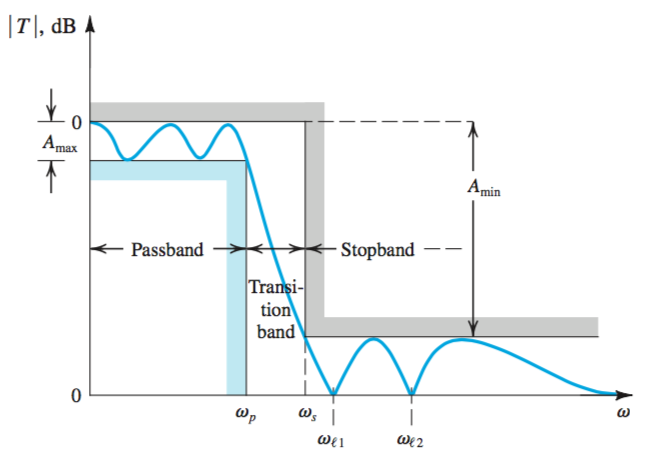
\includegraphics[width=\textwidth]{transmission}

    \begin{equ}[!ht]
        \begin{equation}
            T(s) = \frac{a_1s + a_0}{s + \omega_0}
        \end{equation}
      \caption{General First-Order Transfer Function}
    \end{equ}

    The filter transfer function can be expressed as the ratio of two polynomials in $s$. The degree of the denominator polynomial, $N$, is the filter order. The $N$ roots of the denominator polynomial are the poles (natural modes).

    \subsection{Filter Types}
    \textbf{High Pass} allows high frequencies to pass through (the \textit{passband}) and attenuates frequences below (the \textit{stopband}). \\

    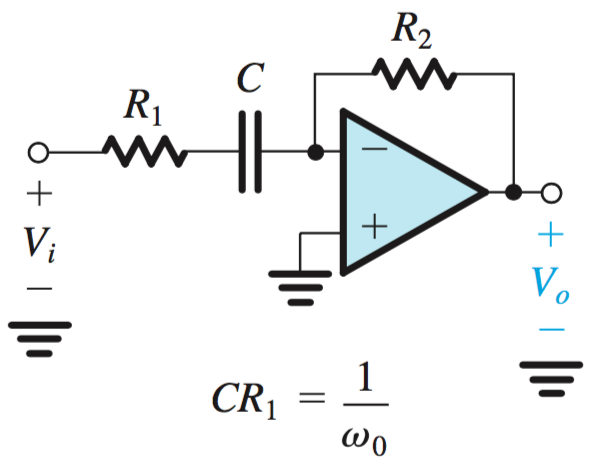
\includegraphics[width=200pt]{highpass} 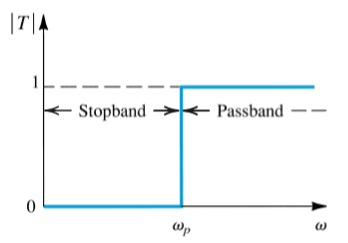
\includegraphics[width=200pt]{highpass2}
    \\
    
    \textbf{Low Pass} allows low frequencies to pass through. \\

    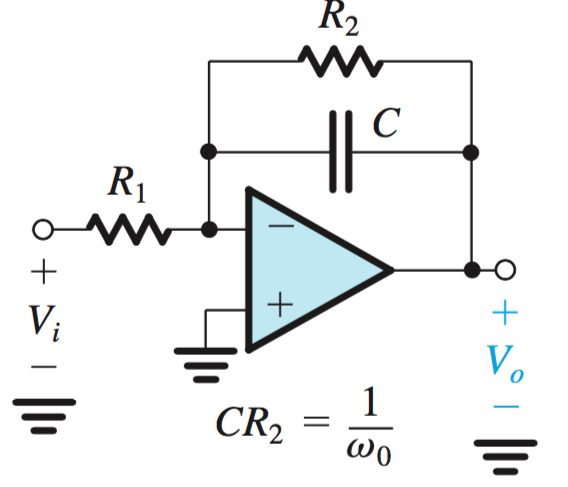
\includegraphics[width=200pt]{lowpass} 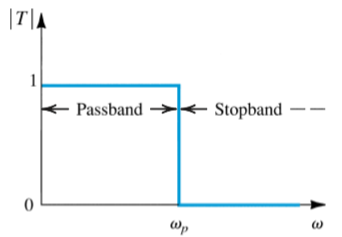
\includegraphics[width=200pt]{lowpass2} 
    
    \pagebreak
     
    
    \textbf{Band Pass} will pass all bands, but invert phase. \\
    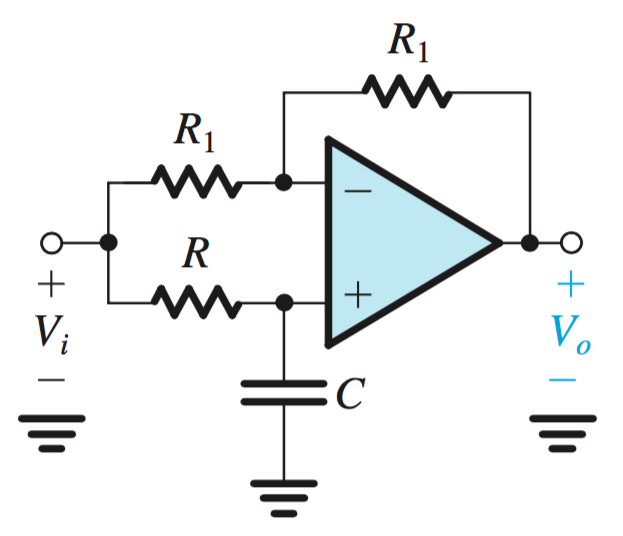
\includegraphics[width=200pt]{allpass} 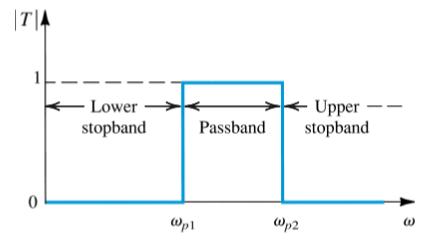
\includegraphics[width=200pt]{bandpass2} 
    \\
    
    \textbf{Band Stop} will stop all bands within the specified range. \\
    
    In each case of attenuation, the slope will be -20 dB per decade. \\
    
    The \textit{All Pass Filter} is a special case which does not attenuate, but serves as a phase shifter, with a unity gain and phase shift at $\omega_0$.
    \subsection{Filter Transmission (2nd Order Filters)}

    \begin{equ}[!ht]
        \begin{equation}
            T(s) = \frac{a_2s^2 + a_1s + a_0}{s^2 + (\omega_0/Q)s + \omega_{0}^2}
        \end{equation}
      \caption{General Second-Order Transfer Function}
    \end{equ}
    \pagebreak

    \subsection{Filter Types}
    \textbf{High Pass} goes zero as the $s$ value goes to zero, and $a_2$ as $s$ goes to $\infty$. \\
    
    $T(s) = \frac{a_0}{s^2 + (\omega_0/Q)s + \omega_{0}^2}$

    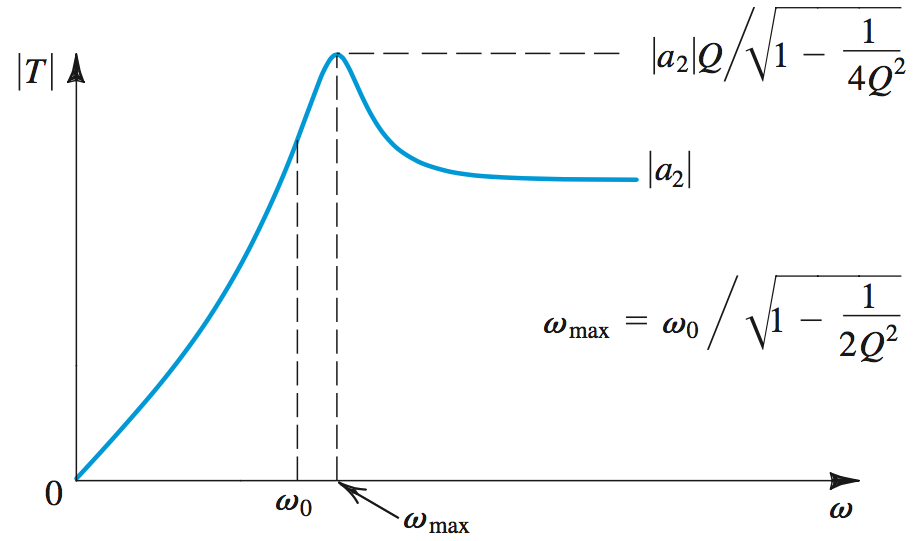
\includegraphics[width=\textwidth]{highpass3}
    \\
    
    \textbf{Low Pass} allows low frequencies to pass through. \\

   $T(s) = \frac{a_2s^2}{s^2 + (\omega_0/Q)s + \omega_{0}^2}$

    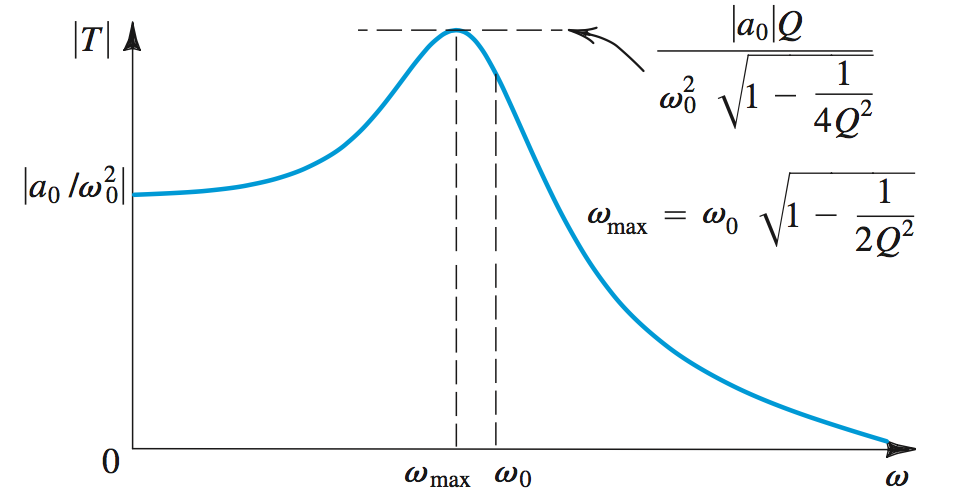
\includegraphics[width=\textwidth]{lowpass3}    
    
    \textbf{Band Pass} will attenuate all but the $\omega_0$ frequency. \\

    $T(s) = \frac{a_1s}{s^2 + (\omega_0/Q)s + \omega_{0}^2}$

    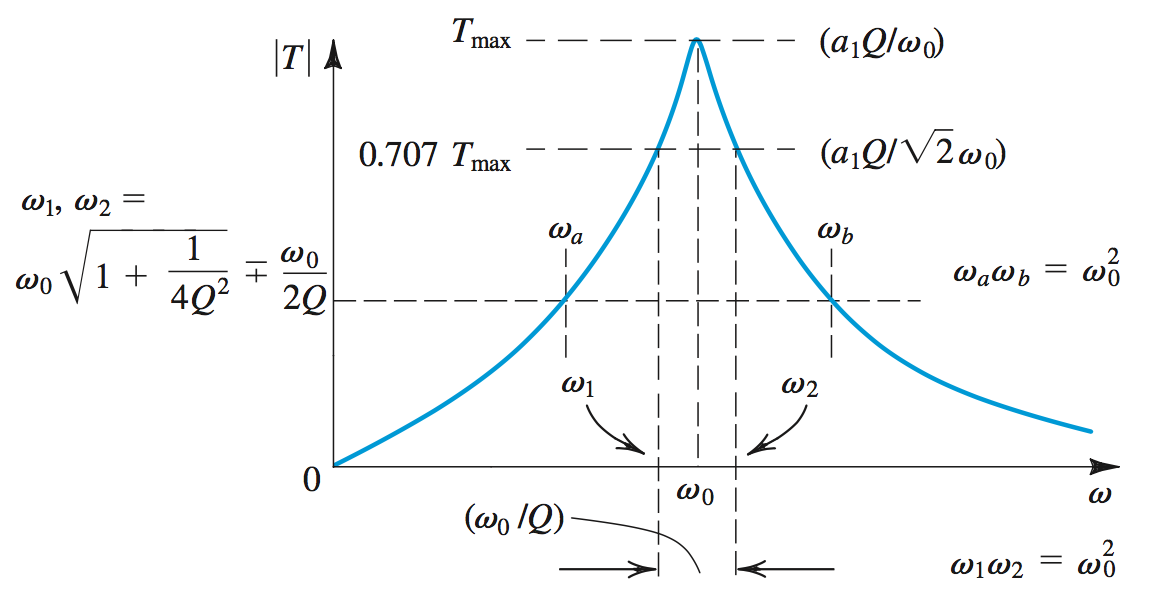
\includegraphics[width=\textwidth]{bandpass3} 
       
    \textbf{Notch} will attenutate at the center frequency $\omega_0$. \\

    $T(s) = a_2\frac{s^2+\omega_{0}^2}{s^2 + (\omega_0/Q)s + \omega_{0}^2}$

    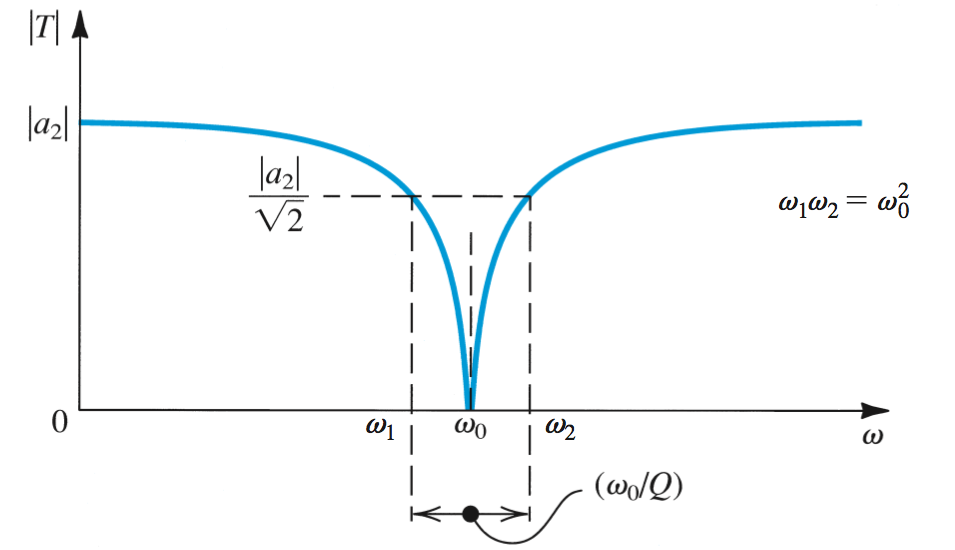
\includegraphics[width=\textwidth]{notch} 
    \\

    $Q = 1/\sqrt{2} = $The Butterworth Maximally Flat Response

    $\text{BW} = \omega_2 - \omega_1 = \omega_0/Q$

    \subsection{Second Order LCR Resonator}

    Resonators are used to realize second order filters.
    
    \begin{center}
        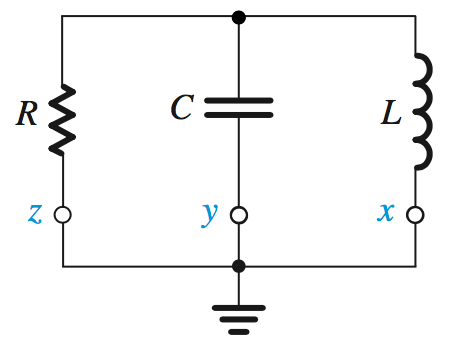
\includegraphics[width=250 px]{resonator} 
    \end{center}    

    For a current applied to this circuit,

    \begin{center}
        $v_0 = I \cdot \frac{1}{Y}$ \\
        
        $\frac{1}{Y} = \frac{1}{\frac{1}{SL} + Cs + \frac{1}{R}}$ \\
                
        $\frac{s/C}{s^2+\frac{s}{CR}+\frac{1}{CL}}$
    \end{center}

    In this case, $\omega_{0}^2 = \frac{1}{CL}$ and $\frac{\omega_0}{Q} = \frac{1}{CR}$

    \begin{center}
            $\omega_0 = 1/\sqrt{LC}$ \\
            
            $Q = \omega_0 CR$
    \end{center}

    Using this structure,

    \begin{center}
        $T(s) = \frac{v_0}{v_i} = \frac{Z_2}{Z_1+Z_2}$
    \end{center}

    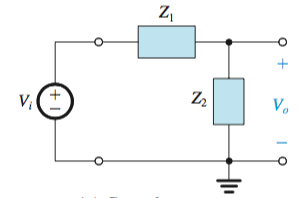
\includegraphics[width=200 px]{res-general} 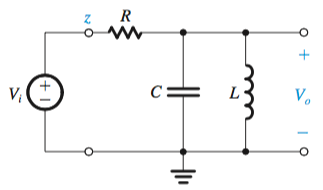
\includegraphics[width=200 px]{res-lpf} \\
    
    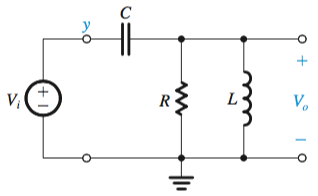
\includegraphics[width=200 px]{res-hpf} 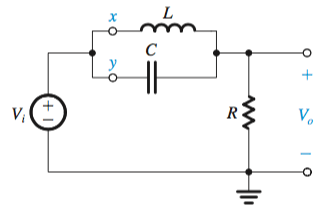
\includegraphics[width=200 px]{res-notch}  \\
    
    By following the structure $T(s) = \frac{v_0}{v_i} = \frac{Z_2}{Z_1+Z_2}$, it can be seen that from these structures the transfer function for each second order filter can be derived by these circuits. It can also be seen that the order of capacitors are mirrored by the single order op amp filters.

    \subsubsection{Antoniou Inductance Circuit}

    Inductors in the resonator circuits can be replaced by a system of op amps, such as the \textit{Antoniou Inducance Simulation Circuit}. \\
    
    From the circuit below, an impedance $Z = sC_4R_1R_3R_5/R_2$, $L = C_4R_1R_3R_5/R_2$

    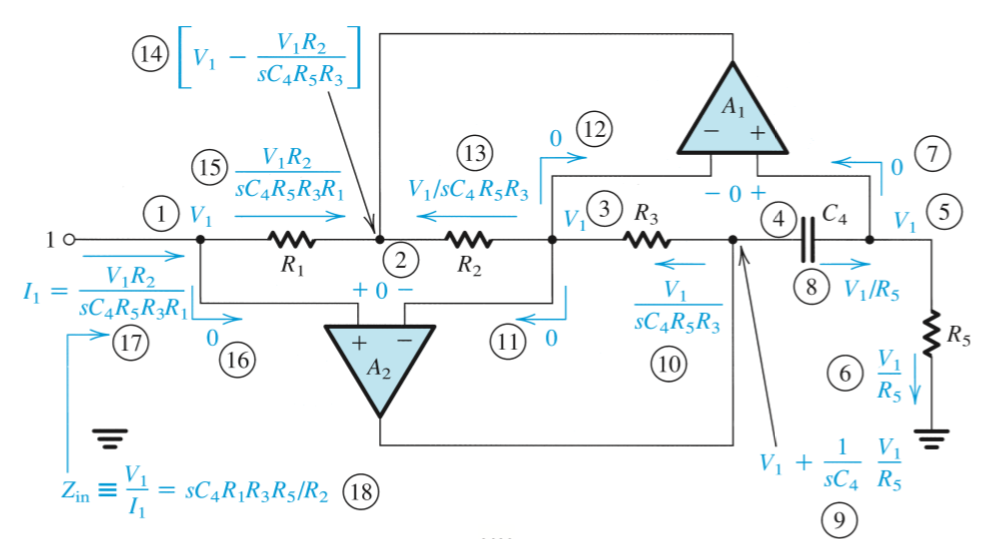
\includegraphics[width=\textwidth]{antoniou}

    The design of this circuit is usually based on selecting $R_1 = R_2 = R_3 = R_5 = R$ and $C_4 = C$, which leads to $L = CR^2$. When used in a resonator,

    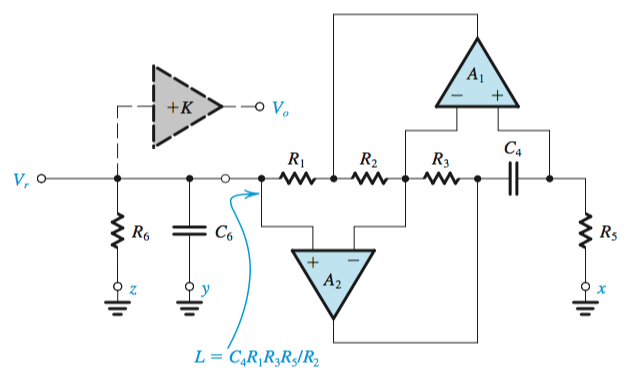
\includegraphics[width=\textwidth]{antoniou-res}

    This circuit would have a pole frequency $\omega_0 = 1/LC_6 = 1/C_4C_6R_1R_3R_5/R_2$ \\
    
    The gain would be derived from $+K$ op amp, $Q = \omega_0C_6R_6$, $\omega_0 = 1/CR$.

    \subsubsection{Filter Types}
    \begin{center}
    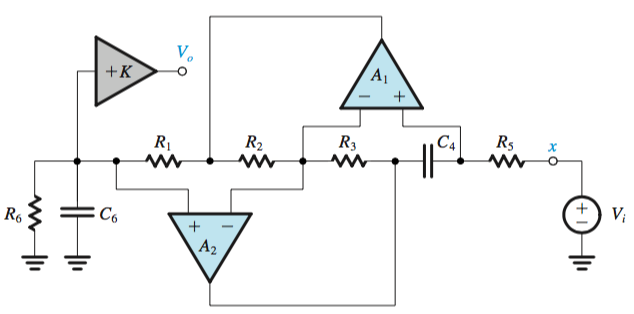
\includegraphics[width=300 px]{lp-antoniou} \\ 

    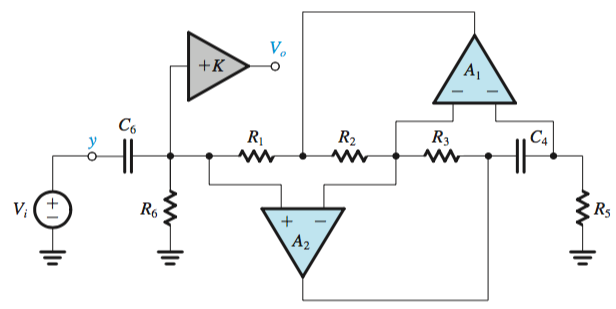
\includegraphics[width=300 px]{hp-antoniou} \\ 
    
    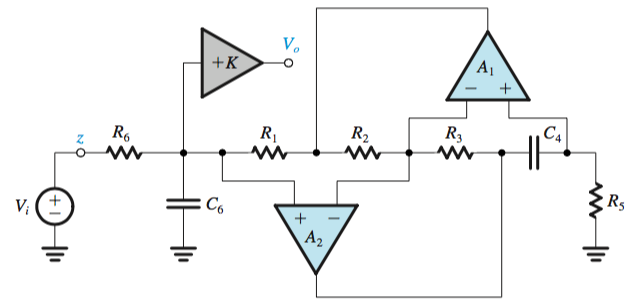
\includegraphics[width=300 px]{bp-antoniou}
    \end{center}

    The position of the capacitor C in each case will mirror the filter type in the first order filters, and in each case the gain will be created through $+K$.

    \subsection{Second Order Active Filters Based on Two Integrators}
    Biquads based on the two-integrator-loop topology are the most versatile and popular second-order filter realizations. There are two varieties: the KHN circuit, which realizes the LP, BP, and HP functions simultaneously and can be combined with the output summing amplifier to realize the notch and all-pass functions; and the Tow–Thomas circuit, which realizes the BP and LP functions simultaneously. Feedforward can be applied to the Tow–Thomas circuit to obtain the circuit, which can be designed to realize any of the second-order functions.
    \subsubsection{KHN Biquad}

    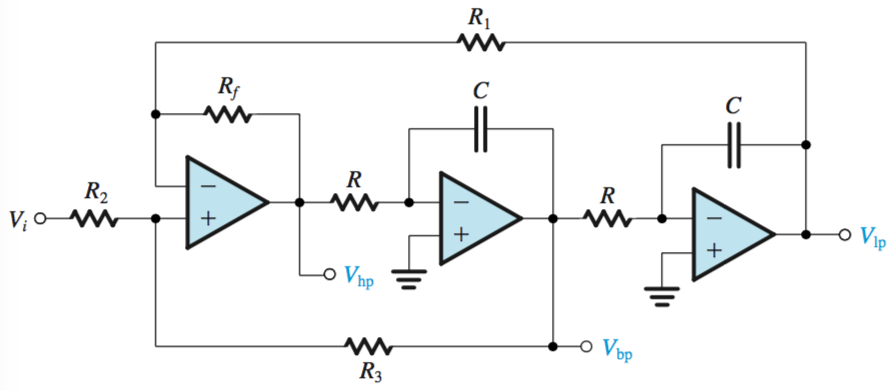
\includegraphics[width=\textwidth]{khn}
    Analyzed by superposition, 
 
    $V_{hp} = \frac{R_3}{R_2+R_3}(1+ \frac{R_f}{R_1})V_i + \frac{R_2}{R_2 + R_3}(1 + R_f)(-\frac{\omega_0}{s} V_{hp}) - \frac{R_f}{R_1}(\frac{\omega_{0}^2}{s^2} V_{hp})$  \\

    Where $R_f/R_1 = 1$, $R_3/R_2 = 2Q - 1$, and $K = 2 - (1/Q)$ \\
     
    Center frequency, $KQ = 2Q - 1$ and $\omega_0 = 1/RC$.
    
    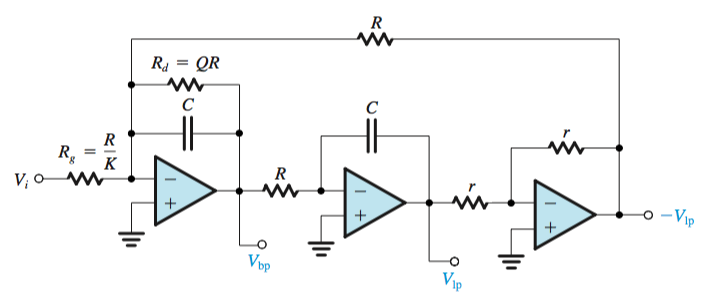
\includegraphics[width=\textwidth]{tow}

    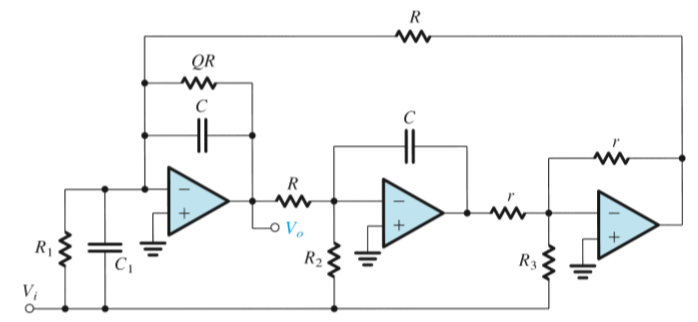
\includegraphics[width=\textwidth]{tow-feed} 

    \subsection{Single Amplifier Biquadratic Active Filters}

    Single-amplifier biquads (\textit{SABs}) are obtained by placing a bridged-T network in the negative-feedback path of an op amp. If the op amp is ideal, the poles realized are at the same locations as the zeros of the $RC$ network. The complementary transformation can be applied to the feedback loop to obtain another feedback loop having identical poles. Different transmission zeros are realized by feeding the input signal to circuit nodes that are connected to ground. SABs are economic in their use of op amps but are sensitive to the op-amp nonidealities and
    are thus limited to low-$Q$ applications ($Q \leq 10$).

    \subsubsection{Bridged T Amplifiers}

    \begin{center}
        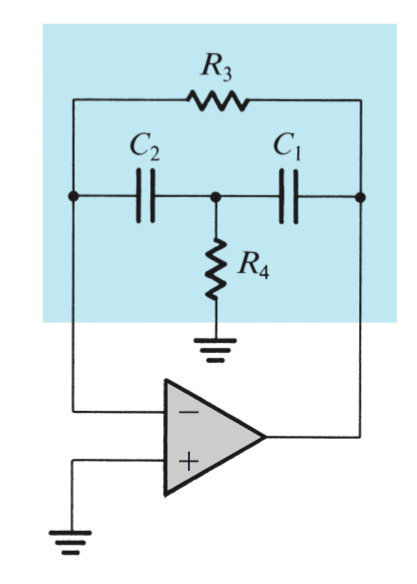
\includegraphics[width=200 px]{bridge-t} 
    \end{center}

    $\omega_0 = 1/\sqrt{C_1C_2R_3R_4}$ \\
    
    $Q = (\frac{\sqrt{C_1C_2R_3R_4}}{R_3})(\frac{1}{C_1}+\frac{1}{C_2})^{-1}$ \\
    
    $m = 4Q^2$ \\
    
    $CR = \frac{2Q}{\omega_0}$ \\

    $R_3 = R$, $R_4 = R/m$

    \subsection{Sensitivity}

    The classical sensitivity function
    $S^{y}_x = \frac{\partial{y}/y}{\partial{x}/x}$
    is a very useful tool in investigating how tolerant a filter circuit is to the unavoidable inaccuracies in component values and to the nonidealities of the op amps.

%%%%%%%%%%%%%%%%%%%%%%%%%%%%%%%%%%%%%%%%%%%%%%%%%

    \section{Signal Generators and Waveform-Shaping Circuits}

    There are two distinctly different types of signal generator: the linear oscillator, which utilizes some form of resonance, and the nonlinear oscillator or function generator, which employs a switching mechanism implemented with a multivibrator circuit.

    \subsection{Oscillator Feedback loop}

    When an output signal is used as input into the $v_+$ terminal of an op amp, a feedback loop is formed where, if the gain is found to be greater than unity, the feedback signal will be summed positively. The feedback and gain loop are then:
    
    \begin{center}
        $A_f(s) = \frac{A(s)}{1-A(2)\beta(s)}$ \\
        
        $L(s) = A(s)\beta(s)$       
    \end{center}
    
    For a feedback loop to produce sinusoidal osciallations at frequency $\omega_0$,

    \begin{center}
        $L(j\omega_0) = A(j\omega_0)\beta(j\omega_0) = 1$
    \end{center}
    
    This is the \textit{Barkhausen criterion}. \\
    

    When analyzing a given oscillator circuit, follow the following steps:

    \begin{enumerate}
        \item Break the feedback loop to determine the loop gain $A(s)\beta(s)$.
        \item The oscillation frequency $\omega_0$ is found as the frequency for which the phase angle of $A(j\omega)\beta(j\omega)$ is zero or, equivalently, 360.
        \item The condition for the oscillations to start is found from \\
        $|A(j\omega_0)\beta(j\omega_0)|$ $\geq 1$
    \end{enumerate}
    \subsubsection{Amplitude Control}
    A popular limiter circuit used to control the amplitude of oscillating circuits is pictured below. By disconnecting the feedback loop, the linear gain $-\frac{R_f}{R_1}$ is found. When the input source goes positive of negative, the limiting value $L_+$ or $L_-$ can be found, as seen in the transfer characteristic. \\
    
    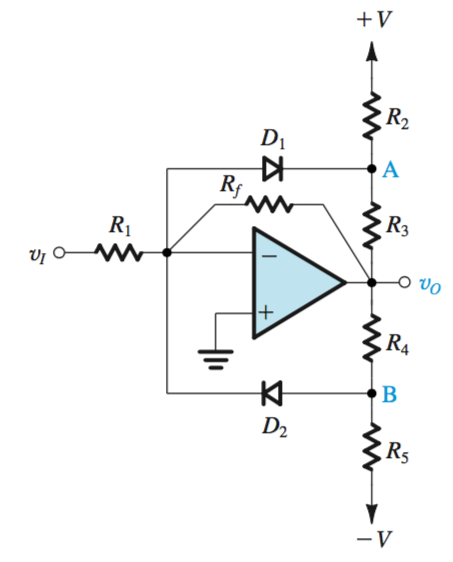
\includegraphics[width = 200 px]{lim} 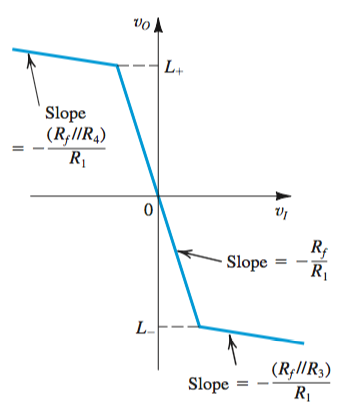
\includegraphics[width = 200 px]{lim-char} 

    \begin{center}
        $L_+ = V\frac{R_4}{R_3} + V_D(1 + \frac{R_4}{R_3})$, $L_- = V\frac{R_3}{R_2} - V_D(1 + \frac{R_3}{R_2})$
    \end{center}

    \subsubsection{Wien Bridge}
    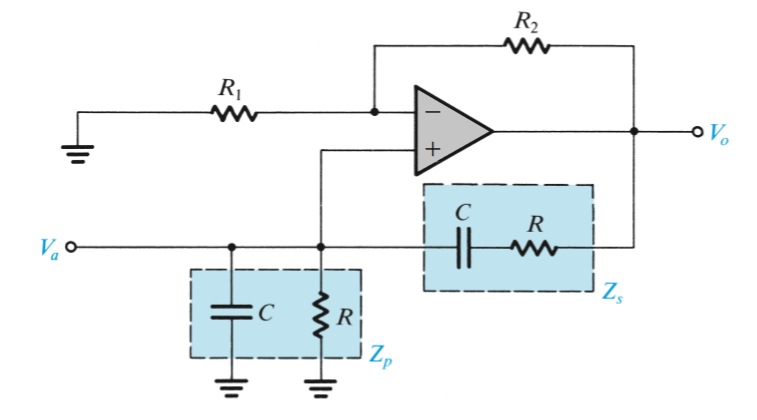
\includegraphics[width = \textwidth]{wien}
    $w_0 = 1/CR$ \\

    $L(s) = (1+\frac{R_2}{R_1})\frac{Z_p}{Z_p+Z_s}$
    
    \subsection{Bistable Multivibrators}
    A bistable multivibrator is an op amp circuit that switches between two stable states indefinitely when it receives a trigger signal. \\
    
    The op amp will saturate at the value $L^+$ or $L^-$, until a value less than, or greater than $L^+\frac{R_1}{R_1+R_2}$ is presented at the inverting input.

    From the transfer characteristics of the non-inverting feedback loop, we can derive this relationship:

    \begin{center}
        $v_+ = v_o \frac{R_1}{R_1+R_2} = L^+\beta$ \\
        
        $L^+\beta - v_I = 0 \rightarrow \textit{no change}$     \\
        
        $L^+\beta - (L^+\beta + 1) = -1 \rightarrow L^-$ \\
        
    \end{center}

    When the $v_I$ value exceeds the other input, it will trigger a positive feedback loop which fixes the op amp at its positive or negative saturation. \\
    
    This pair of values in the negative and positive direction are the $V_{TH}$ and $V_{TL}$, which can be found to be $L^+\beta$ and $L^-\beta$.
    
    \begin{center}
        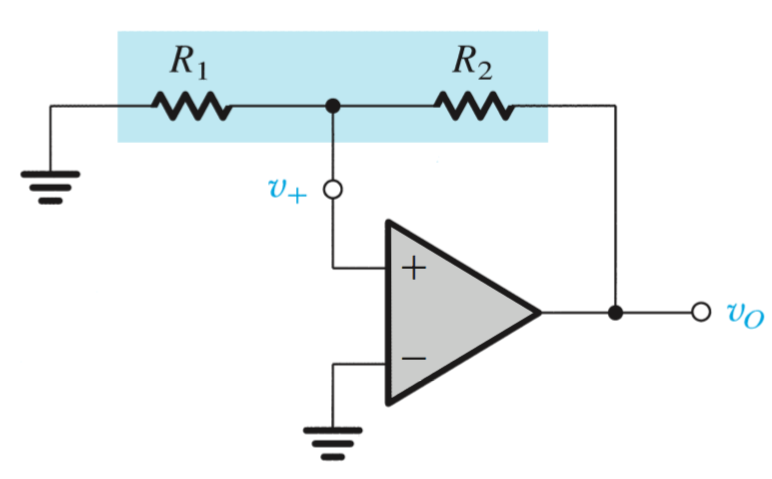
\includegraphics[width = 300 px]{bistable}        
    \end{center}
    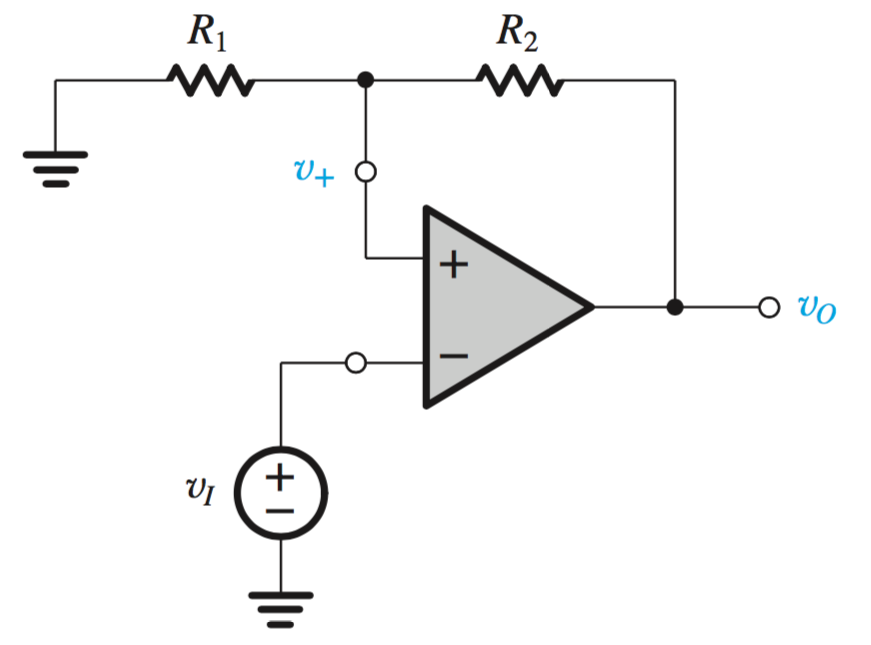
\includegraphics[width = 200 px]{bistable-neg} 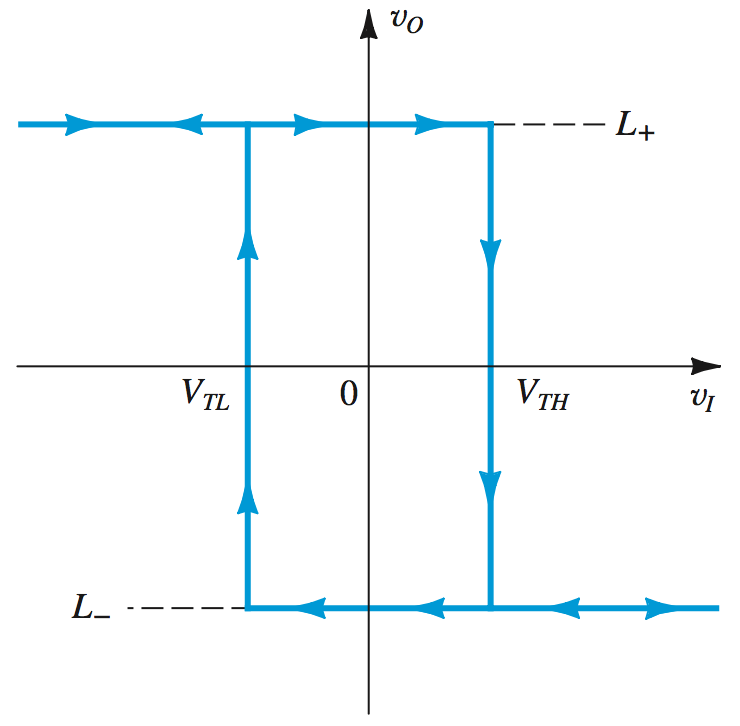
\includegraphics[width = 200 px]{bistable-neg-char} \\
    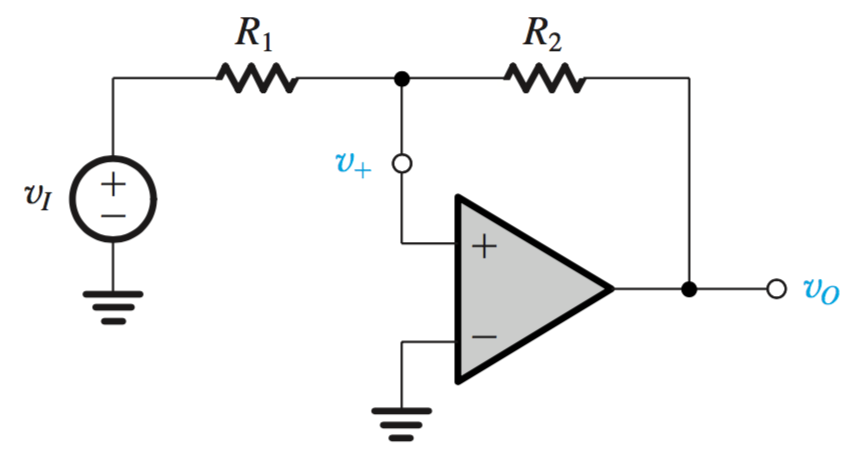
\includegraphics[width = 200 px]{bistable-pos} 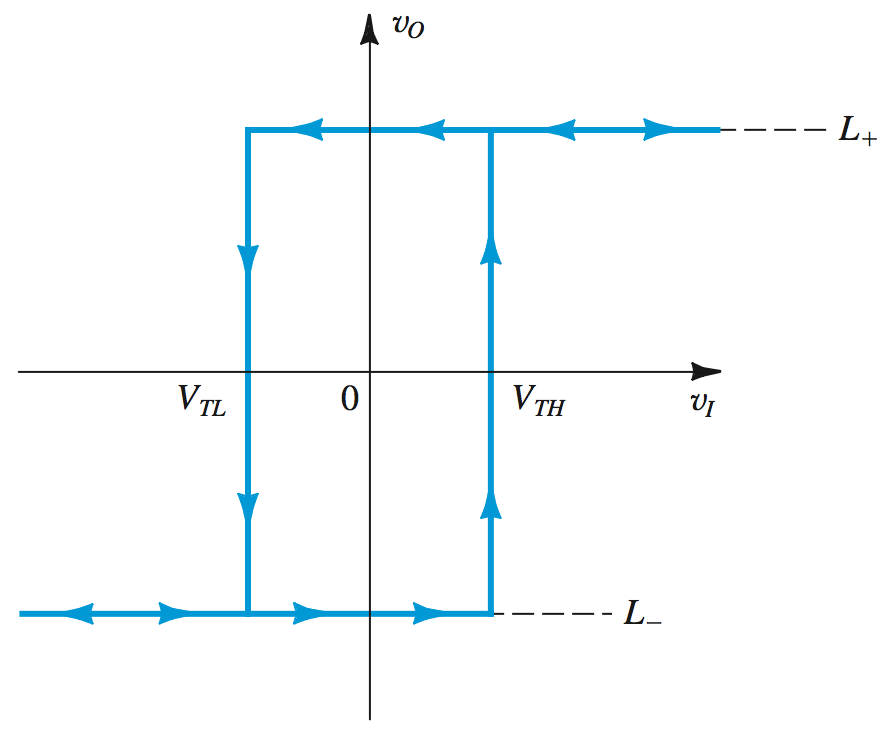
\includegraphics[width = 200 px]{bistable-pos-char} \\
    
    For the non-inverting bistable circuit, superposition must be used to find the value of $v^+$ due to the input $v_I$ and the output $v_o$ being fed back into the op amp. Therefore,

    \begin{center}
        $v^+ = v_I\frac{R_2}{R_1+R_2} + v_o\frac{R_1}{R_1+R_2}$
    \end{center}

    To find the $V_{TH}$ and $V_{TL}$ for this circuit, we must find values that create make $v^+$ less than zero. Assuming the state that this will happen, set $v_o$ to $L^+$, $v^+$ to $0$, and $v_I$ to $V_{TL}$. Rearranging and solving for $V_{TL}$,
    
    \begin{center}
        $V_{TL} = -L_+\frac{R_1}{R_2}$
    \end{center}

    This technique can be used to find the $V_{TH}$ as well, by rewriting for $L_+$.

    \begin{center}
        $V_{TH} = -L_-\frac{R_1}{R_2}$
    \end{center}

    For each case, adding a reference DC voltage $V_R$ to an input will move the characteristic horizontally by a value of $V_R$, as the $v_I$ input must now match $L^+\beta + V_R$, for example.
    \subsection{Astable Multivibrators}
    By connecting a bistable multivibrator with an RC circuit in a feedback loop, a square wave can be generated where the circuit will switch states periodically. The capacitor will charge until it reaches $\beta L^+$, then discharge until $\beta L^-$, upon which time it will begin charging again.

    \begin{center}
        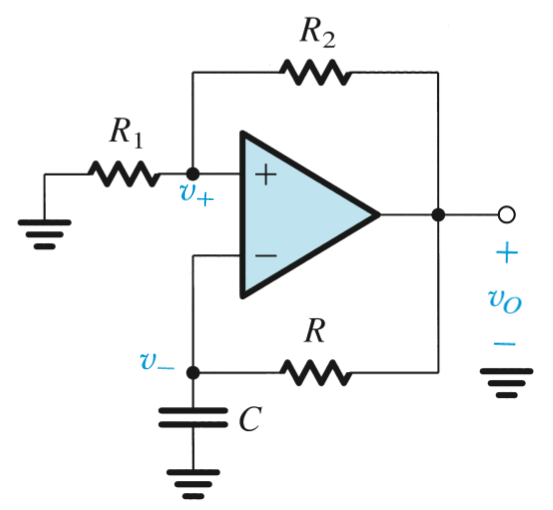
\includegraphics[width = 250 px]{astable}        
    \end{center}

    The time constant for this circuit is $\tau = CR$, which will define the period.

    \begin{center}
        $T = 2\tau \text{ln}\frac{1+\beta}{1-\beta}$
    \end{center}

    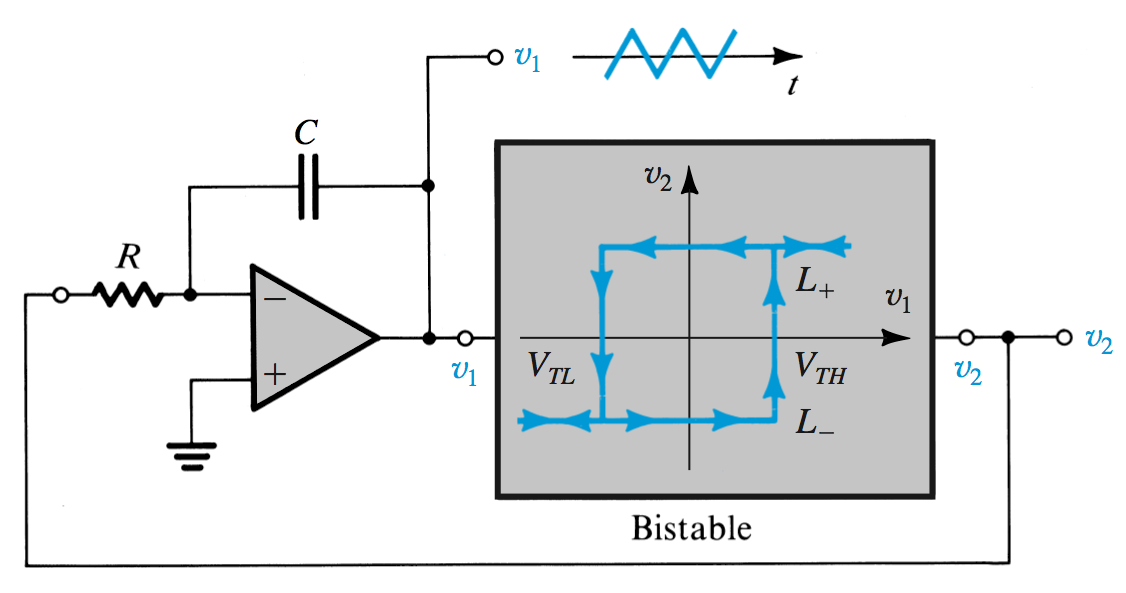
\includegraphics[width = 350 px]{triangle}  
    
    \begin{center}
        $T_1 = CR\frac{V_{TH}-V_{TL}}{L^+}$
        $T_2 = CR\frac{V_{TH}-V_{TL}}{L^-}$
    \end{center}

    \subsection{Monostable Multivibrator}

    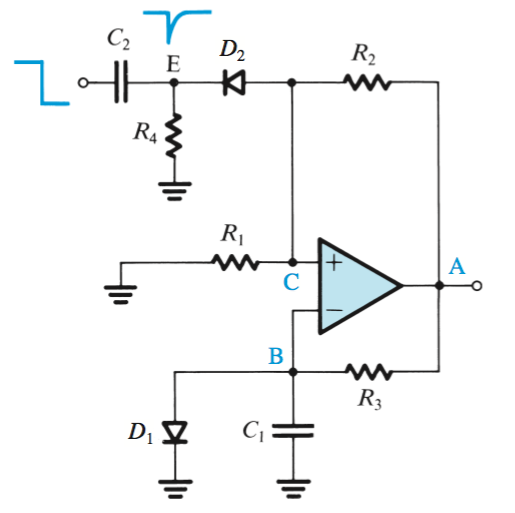
\includegraphics[width = 200 px]{mono} 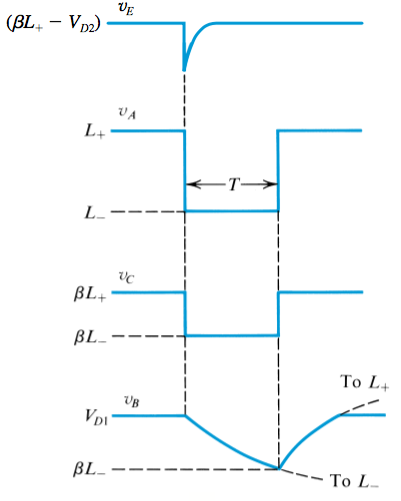
\includegraphics[width = 200 px]{mono-char}        

    A single pulse seen at point $E$ will trigger $L_-$ saturation, where point $B$ will be pulled through the capacitor, as the negative voltage turns off $D_1$. \\
    
    After the period $T$, the circuit will saturate to $L_+$ again, upon which point it will stabilize until the next pulse. 

    \subsection{Precision Rectifiers}
    
    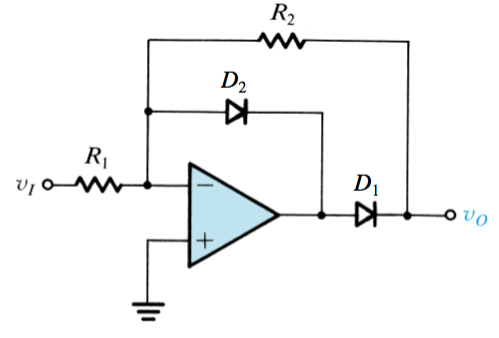
\includegraphics[width = 200 px]{prec1} 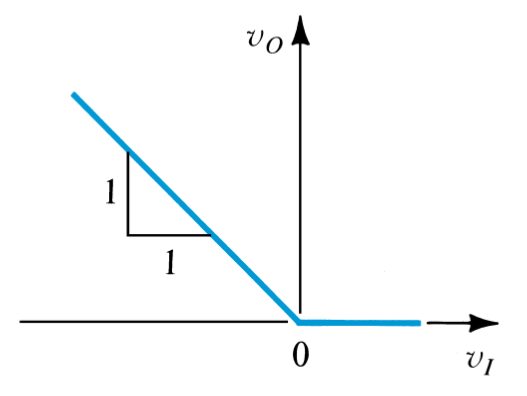
\includegraphics[width = 200 px]{prec-char}  
    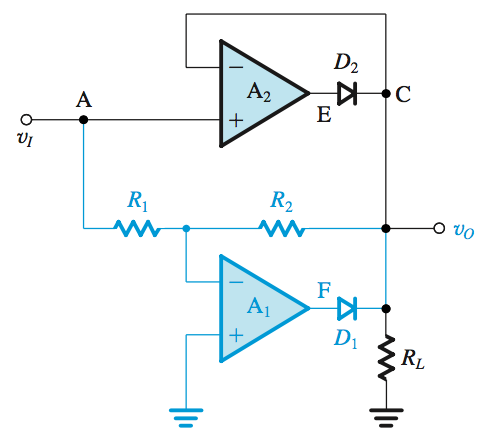
\includegraphics[width = 200 px]{prec-full} 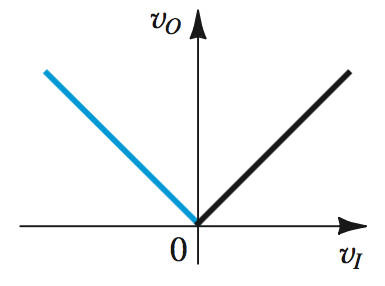
\includegraphics[width = 200 px]{prec-full-char}

    \end{document}